% WebContactsProPlus — UML-ish class diagram
\documentclass[border=12pt]{standalone}
\usepackage{tikz}
\usetikzlibrary{positioning, arrows.meta, shapes.multipart, calc, fit, backgrounds}

\begin{document}
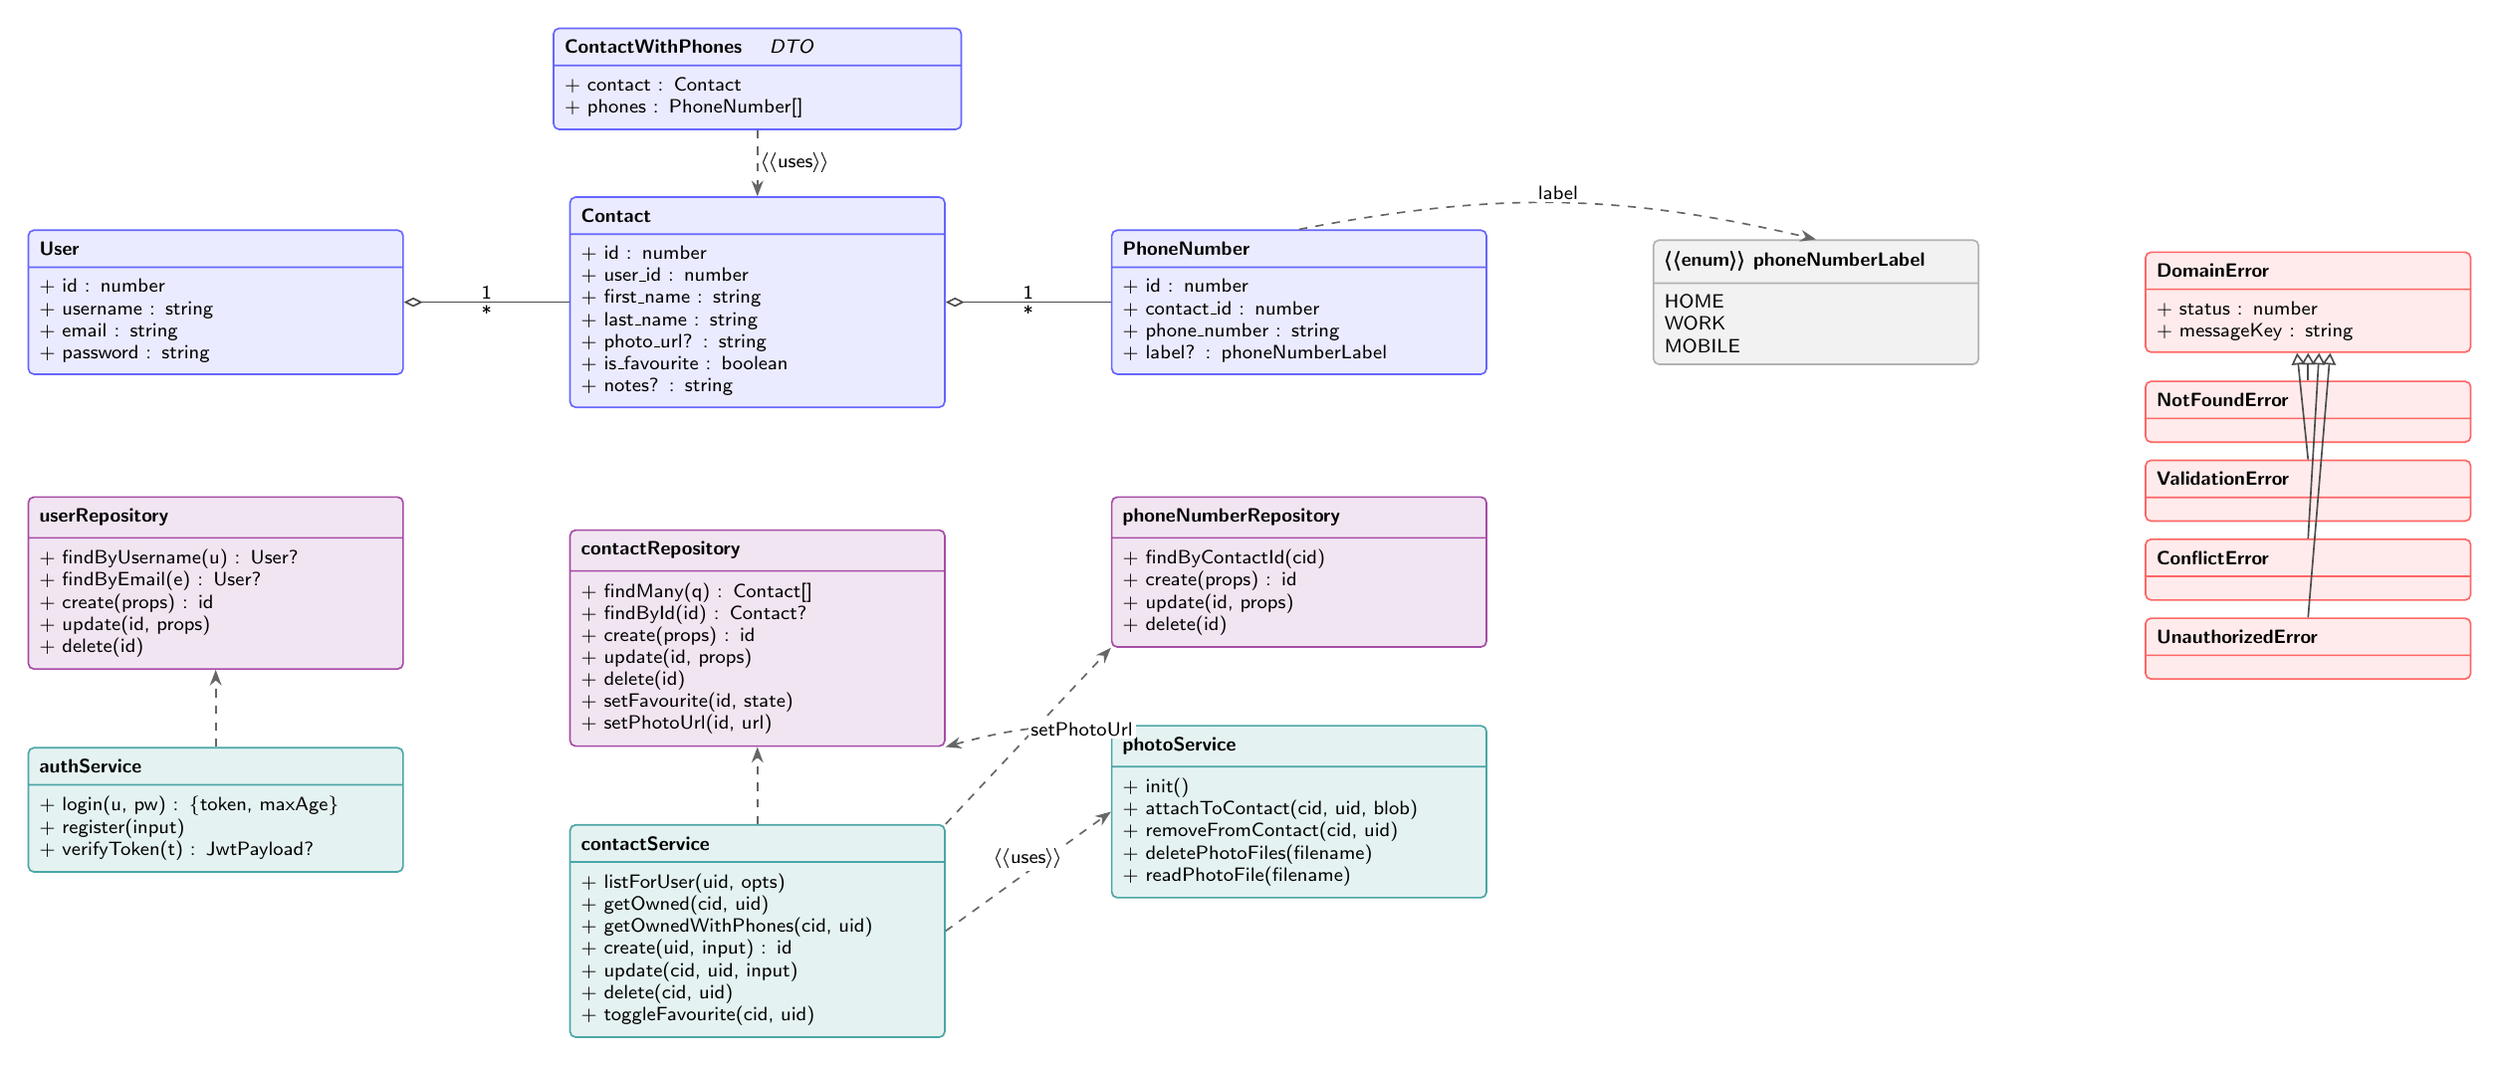
\begin{tikzpicture}[
    >=Stealth,
    font=\sffamily\footnotesize,
    node distance=28pt and 60pt,
    cls/.style={
        rectangle split, rectangle split parts=2, draw, line width=0.6pt,
        rectangle split draw splits=true,
        text width=128pt,
        rectangle split part align={center, left},
        rounded corners=2pt,
        inner sep=4pt,
        font=\sffamily\scriptsize,
    },
    entity/.style={cls, fill=blue!8,    draw=blue!60},
    service/.style={cls, fill=teal!10,  draw=teal!70},
    repo/.style={cls, fill=violet!10,   draw=violet!70},
    err/.style={cls, fill=red!8,        draw=red!60, text width=110pt},
    enum/.style={cls, fill=gray!10,     draw=gray!60, text width=110pt},
    comp/.style={-{Diamond[open]}, line width=0.6pt, draw=black!70},
    dep/.style={->, line width=0.6pt, dashed, draw=black!60},
    inherit/.style={-{Triangle[open]}, line width=0.6pt, draw=black!70},
    mult/.style={font=\sffamily\scriptsize, fill=white, inner sep=1pt},
]

% ===================== Row 1: entities =====================
\node[entity] (user) {
    \textbf{User}
    \nodepart{second}
    + id : number \\
    + username : string \\
    + email : string \\
    + password : string
};

\node[entity, right=of user] (contact) {
    \textbf{Contact}
    \nodepart{second}
    + id : number \\
    + user\_id : number \\
    + first\_name : string \\
    + last\_name : string \\
    + photo\_url? : string \\
    + is\_favourite : boolean \\
    + notes? : string
};

\node[entity, right=of contact] (phone) {
    \textbf{PhoneNumber}
    \nodepart{second}
    + id : number \\
    + contact\_id : number \\
    + phone\_number : string \\
    + label? : phoneNumberLabel
};

% Enum to the right of PhoneNumber
\node[enum, right=of phone] (enum) {
    \textbf{\textlangle\textlangle enum\textrangle\textrangle{} phoneNumberLabel}
    \nodepart{second}
    HOME \\ WORK \\ MOBILE
};

% ===================== Row 2: repositories =====================
\node[repo, below=44pt of user] (userrepo) {
    \textbf{userRepository}
    \nodepart{second}
    + findByUsername(u) : User? \\
    + findByEmail(e) : User? \\
    + create(props) : id \\
    + update(id, props) \\
    + delete(id)
};

\node[repo, below=44pt of contact] (contactrepo) {
    \textbf{contactRepository}
    \nodepart{second}
    + findMany(q) : Contact[] \\
    + findById(id) : Contact? \\
    + create(props) : id \\
    + update(id, props) \\
    + delete(id) \\
    + setFavourite(id, state) \\
    + setPhotoUrl(id, url)
};

\node[repo, below=44pt of phone] (phonerepo) {
    \textbf{phoneNumberRepository}
    \nodepart{second}
    + findByContactId(cid) \\
    + create(props) : id \\
    + update(id, props) \\
    + delete(id)
};

% ===================== Row 3: services =====================
\node[service, below=of userrepo] (authsvc) {
    \textbf{authService}
    \nodepart{second}
    + login(u, pw) : \{token, maxAge\} \\
    + register(input) \\
    + verifyToken(t) : JwtPayload?
};

\node[service, below=of contactrepo] (contactsvc) {
    \textbf{contactService}
    \nodepart{second}
    + listForUser(uid, opts) \\
    + getOwned(cid, uid) \\
    + getOwnedWithPhones(cid, uid) \\
    + create(uid, input) : id \\
    + update(cid, uid, input) \\
    + delete(cid, uid) \\
    + toggleFavourite(cid, uid)
};

\node[service, below=of phonerepo] (photosvc) {
    \textbf{photoService}
    \nodepart{second}
    + init() \\
    + attachToContact(cid, uid, blob) \\
    + removeFromContact(cid, uid) \\
    + deletePhotoFiles(filename) \\
    + readPhotoFile(filename)
};

% ===================== DTO (above contact, off to the side) =====================
\node[entity, above=24pt of contact, text width=140pt] (cwp) {
    \textbf{ContactWithPhones} \quad {\scriptsize\textit{DTO}}
    \nodepart{second}
    + contact : Contact \\
    + phones : PhoneNumber[]
};

% ===================== Errors (far right, vertical column) =====================
\node[err, right=of enum] (domainerr) {
    \textbf{DomainError}
    \nodepart{second}
    + status : number \\
    + messageKey : string
};
\node[err, below=10pt of domainerr] (notfound)     {\textbf{NotFoundError}      \nodepart{second}~};
\node[err, below=6pt of notfound]   (validation)   {\textbf{ValidationError}    \nodepart{second}~};
\node[err, below=6pt of validation] (conflict)     {\textbf{ConflictError}      \nodepart{second}~};
\node[err, below=6pt of conflict]   (unauth)       {\textbf{UnauthorizedError}  \nodepart{second}~};

% ===================== Relationships =====================
% Composition: User 1 ─◇ Contact *
\draw[comp] (contact.west) -- node[mult, above]{1} node[mult, below]{*} (user.east);
% Composition: Contact 1 ─◇ PhoneNumber *
\draw[comp] (phone.west)   -- node[mult, above]{1} node[mult, below]{*} (contact.east);

% DTO uses Contact + PhoneNumber (dashed)
\draw[dep] (cwp.south) -- node[mult, right]{\textlangle\textlangle uses\textrangle\textrangle} (contact.north);

% PhoneNumber.label : phoneNumberLabel (label arrow above the boxes)
\draw[dep] (phone.north) to[bend left=12] node[mult, above]{label} (enum.north);

% Services -> their repositories (vertical, dashed)
\draw[dep] (authsvc.north)    -- (userrepo.south);
\draw[dep] (contactsvc.north) -- (contactrepo.south);

% contactService also depends on phoneNumberRepository (cross-link)
\draw[dep] (contactsvc.north east) -- (phonerepo.south west);

% contactService → photoService (cascade)
\draw[dep] (contactsvc.east) -- node[mult, above]{\textlangle\textlangle uses\textrangle\textrangle} (photosvc.west);

% photoService → contactRepository (setPhotoUrl)
\draw[dep] (photosvc.north west) to[bend right=8] node[mult, right]{setPhotoUrl} (contactrepo.south east);

% Error hierarchy (open-triangle inheritance arrows)
\draw[inherit] (notfound.north)    -- (domainerr.south);
\draw[inherit] (validation.north)  -- ($(domainerr.south)+(-4pt,0)$);
\draw[inherit] (conflict.north)    -- ($(domainerr.south)+(4pt,0)$);
\draw[inherit] (unauth.north)      -- ($(domainerr.south)+(8pt,0)$);

\end{tikzpicture}
\end{document}
